% FUNDAMENTAÇÃO TEÓRICA--------------------------------------------------------

\chapter{FUNDAMENTAÇÃO TEÓRICA}
\label{chap:fundamentacao-teorica}

Neste capítulo, serão abordados os aspectos teóricos necessários para o melhor discernimento das definições e componentes a serem utilizados ao longo do projeto. De início, serão abordados os conceitos base como redes \textit{Wireless}, \textit{Internet of Things}, \textit{Smart Things} e o protocolo \textit{MQTT}. Conceitos como a montagem de circuitos eletrônicos, sensoriamento, implementação de sistemas embarcados assim como as tecnologias envolvidas na criação de aplicações \textit{mobile} e \textit{desktop} também serão tratadas neste capítulo. As subseções posteriores, agruparão os conceitos em elementos: de base, de \textit{Hardware},  de \textit{Firmware} e de \textit{Software}.  

\section{Elementos Base}

\subsection{Redes \textit{Wireless}}

O termo \textit{Wireless} provém do inglês: \textit{wire} (fio, cabo); less (sem); caracteriza qualquer tipo de conxexão para transmissão de sem a utilização fios ou cabos \cite{redeswireless}. É importante definir que uma rede sem fio possibilita um conjunto de equipamentos conectados através de sinais de rádio frequência possuindo vantagens cruciais para a aplicação do conceito de Internet das Coisas:

\begin{itemize}
	\item \textbf{Maior produtividade - } disponibiliza acesso à rede em todo o raio de alcance onde o ponto de acesso está instalado, oferecendo liberdade de deslocamento com conexão contínua;
	
	\item \textbf{Flexibilidade de instalação -} podem ser instaladas em locais com temperaturas elevadas, em que os cabos não suportariam, ou em locais que necessitam de acesso temporário;
	
	\item \textbf{Redução de custo - } reduzem os custos de instalação, dispensando o uso de material para cada ponto de conexão;
	
	\item \textbf{Interoperabilidade e segurança - } capaz de comunicar sistemas de forma confiável e com segurança, possuindo chaves de acesso e até mesmo transferindo mensagens criptografadas.   

\end{itemize}

Dentre as diversas características podemos destacar que as redes \textit{wireless} são dividas quanto a \textbf{abrangência de sinal} em:

\begin{itemize}
	\item \textbf{\textit{Wireless Local Area Network} - WLAN - } rede de área local;
	\item \textbf{\textit{Wireless Metropolitan Area Network} - WLAN - } rede de região metropolitana;
	\item \textbf{\textit{Wireless Wide Area Network} - WWAN - } rede de área mundial sem fio;
	\item \textbf{\textit{Wireless Local Loop} - WLL - } acesso fixo sem fio;
	\item \textbf{\textit{Wireless Personal Area Network} - WPAN} - redes pessoais sem fio;
\end{itemize}


O grupo de trabalho \textit{Institute of Electrical and Electronics Engineers} - \textit{IEEE} 802.11\textit{ Wireless LAN}, fundado em 1987, realizou a padronização das \textit{WLANs}. Desenvolveu-se o padrão DS-SS IEEE 802.11b, chamado de \textit{Wi-Fi} pela \textit{Wireless Ethernet Compatibility Alliance} - WECA o qual é amplamente usado no mercado atual. \cite{internetdascoisassemmisterios}. A partir dessa padronização é possível aplicar as transmissões de dados por diversos protocolos de maneira barata e prática.

A topologia de uma rede IEEE 802.11 (\textit{Wi-Fi})  possui os seguintes elementos-chave:

\begin{itemize}
	\item \textbf{BSS - \textit{Basic Service Set} -} corresponde a uma célula de comunicação \textit{wireless};
	\item \textbf{STA - \textit{Stations} -} são as estações de trabalho que comunicam-se entre si dendo da \textbf{BSS};
	\item \textbf{AP - \textit{Access Point} -} coordena a comunicação entre as \textbf{STA's} dentro da \textbf{BSS}. Na maioria das vezes roteadores realizam tal operação;
	\item \textbf{\textit{Bridge} -} faz a ligação entre diferentes redes, por exemplo, uma rede sem fio para uma rede cabeada convencional;
	\item  \textbf{ESS - \textit{Estended Service Set} -} consiste de várias células \textbf{BSS's} vizinhas que se interceptam e cujos \textbf{AP's} estão conectados a uma mesma rede tradicional. Nestas condições uma \textbf{STA} pode movimentar-se de um \textbf{BSS} para outr, permanecendo conectada à rede. Este processo é denominado \textit{Roaming}.
\end{itemize}

\subsection{A Internet das Coisas}

Existem divergências em relação ao conceito de Internet das Coisas (\textit{Internet of Things - IoT}), sendo que todos os conceitos, em resumo, fazem alusão à um conjunto de tecnologias e protocolos associados que permitem que objetos se conectem a uma rede de comunicações e onde são identificados e controlados.
Com o \textit{IoT} surge a \textit{hiperconectividade} a qual possibilita a aquisição de uma grandeza de informações as quais podem ser utilizadas para melhorar um processo, produto ou serviço.


\section{Elementos de \textit{Hardware}}
\subsection{O microcontrolador ESP8266}

O \textit{ESP8266} (\autoref{fig:esp8266ex}) é um chip microcontrolador da fabricante chinesa \textit{Espressif Systems}. Construído em torno de um processador Tensilica Xtensa LX3, inclui \textit{Wi-Fi on-board}. Originalmente concebido como um adaptador \textit{UART} para \textit{Wi-Fi} (utilizado em \textit{tablets}), permitindo que outros microcontroladores se conectem a uma rede \textit{Wi-Fi} e façam conexões \textit{TCP/IP} simples usando comandos do estilo \textit{Hayes}, o \textit{ESP8266} rapidamente se tornou popular como um microcontrolador autônomo devido ao seu ponto de preço baixo.

\begin{figure}[H]
	\centering
	\caption{\textit{ESP8266EX}.}
	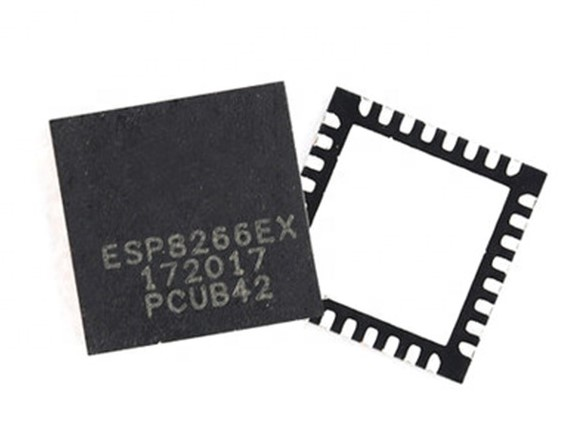
\includegraphics[width=0.3\textwidth]{figuras/esp8266ex.jpg}
	\fonte{DIGIKEY, 2020}
	\label{fig:esp8266ex}
\end{figure} 

Apesar da falta de documentação inicial, uma grande comunidade foi formada em
torno do ESP8266, e a comunidade integrou e deu suporte ao \textit{firmware} para o chip, fazendo-o compatível com a plataforma \textit{Arduino}.
Embora o chip \textit{ESP8266} seja feito pela \textit{Espressif}, existem diversos módulos criados para aplicações distintas (\autoref{fig:modulos_esp8266}).

\begin{figure}[H]
	\centering
	\caption{Alguns exemplos de módulos com base no \textit{ESP8266EX}.}
	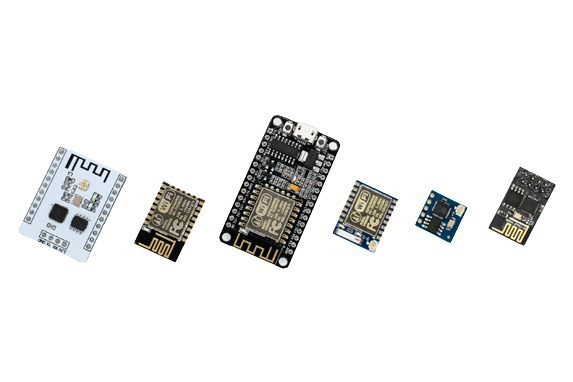
\includegraphics[width=0.5\textwidth]{figuras/modulos_esp8266.png}
	\fonte{FILIPEFLOP, 2020 [adaptado]}
	\label{fig:modulos_esp8266}
\end{figure} 

Os modelos podem se diferenciar pela quantidade de pinos extenados, memória \textit{flash} instalada, modelo de antena, entre outros. Para a realização deste trabalho foram escolhidos os modelos: \textit{ESP-12S} (\autoref{fig:esp12s}) e \textit{ESP-12E} (\autoref{fig:esp12e}). Ambos possuem 11 {GPIOs - General Purpose Input Output} sendo ideais para a leitura de uma gama de sensores. A diferença entre ambos está no desenho da antena integrada, sendo a do ESP-12S mais otimizada, e na quantidade de pinos externados, o ESP-12S não extena os pinos voltados para conexão \textit{SPI} e de cartões \textit{SD}. As características gerais e específicas para o densenvolvimento deste trabalho estão descritas no \textbf{anexo A}. 


\begin{figure}[H]
	\centering
	\caption{Vista superior do \textit{ESP-12S}.}
	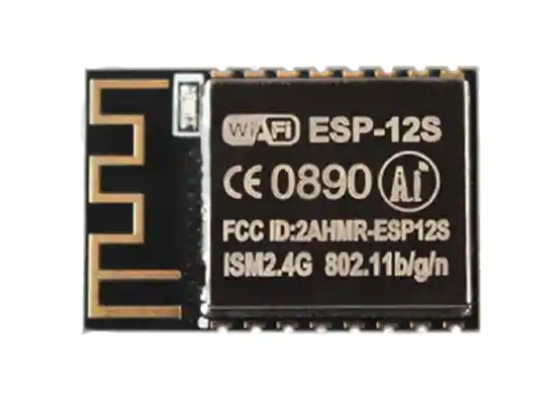
\includegraphics[width=0.3\textwidth]{figuras/ESP-12S.png}
	\fonte{FILIPEFLOP, 2020}
	\label{fig:esp12s}
\end{figure} 

\begin{figure}[H]
	\centering
	\caption{Vista superior do \textit{ESP-12E}.}
	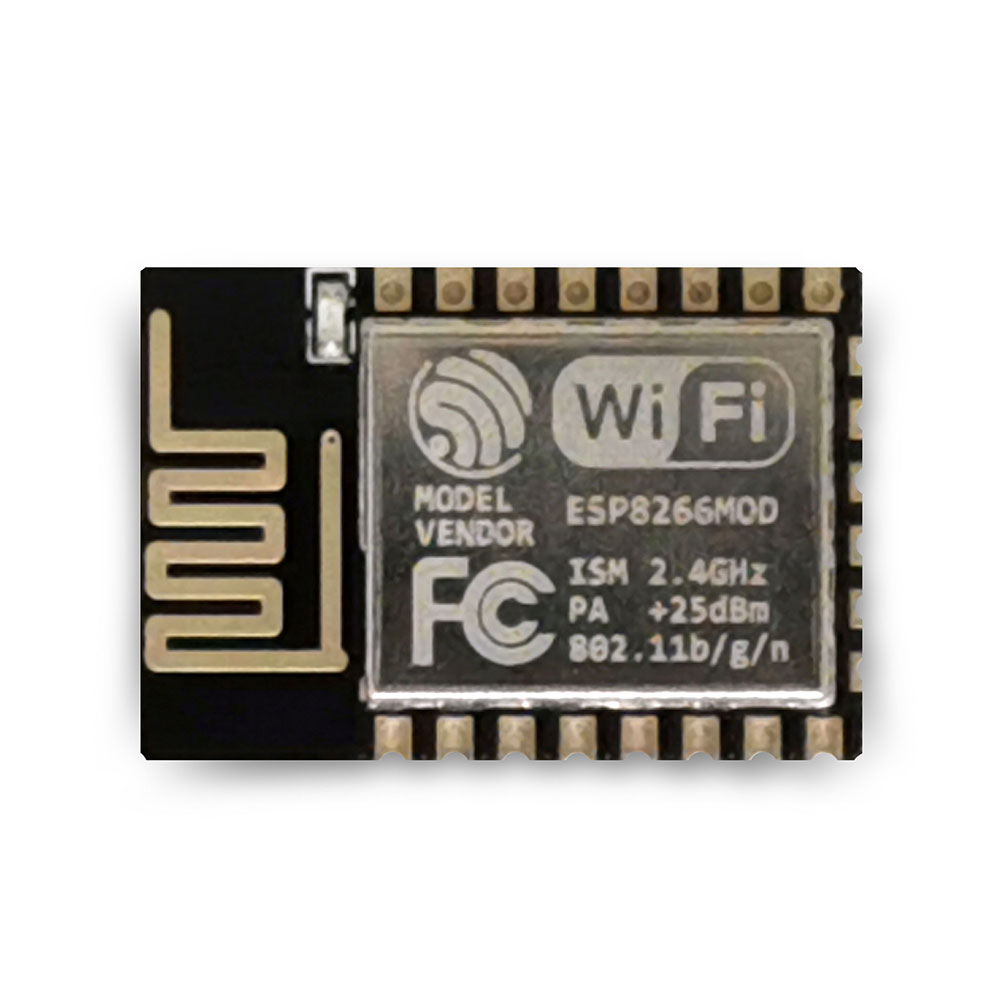
\includegraphics[width=0.3\textwidth]{figuras/ESP-12E.png}
	\fonte{FILIPEFLOP, 2020}
	\label{fig:esp12e}
\end{figure} 



\subsection{A Raspberry Pi Zero W}

A \textit{Raspberry Pi Zero W} é basicamente um computador de placa única. Ela possui recursos como \textit{slot} para cartão \textit{microSD}, conectores \textit{HDMI} e de câmera, conectividade \textit{Wi-Fi} e \textit{Bluetooth 4.0}, um conector macho de entrada-saída (\textit{GPIO}) de 40 pinos e mini conector de alimentação \textit{+ 5VDC}. O microcontrolador baseado no processador \textit{BCM2835 ARMv7 system-on-chip (SoC)} alimenta o Pi Zero W.

Essa versão de \textit{Hardware} é muito compacta, ficando no meio termo entre as fazes de prototipação e aplicação. Com o microprocessador \textit{ARM BCM2835} de \textit{1GHz}, memória \textit{RAM} de \textit{512MB} e um sistema operacional enxuto instalado, a Raspberry Pi Zero W é ideal para rodar aplicações como um \textit{Broker MQTT}. Informações adicionais estão disponíveis no \textbf{Anexo B}.

\begin{figure}[H]
	\centering
	\caption{Vista superior da \textit{Raspberry Pi Zero W}}
	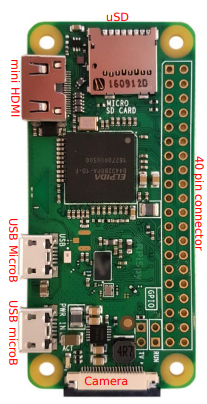
\includegraphics[width=0.3\textwidth, angle = 90]{figuras/rasp_zerow.png}
	\fonte{SPARKFUN, 2020}
	\label{fig:rasppizerow}
\end{figure} 

\subsection{As fontes de alimentação DC}

Para alimentação elétrica de todos os dispositivos eletrônicos envolvidos no processo de automação da cisterna, foram utilizadas dois tipos de fontes chaveadas: de \textit{12V/20A} para o módulo \textbf{CCM} e \textit{12V/10A} para o módulo \textbf{TCM}, representadas pela \autoref{fig:fontechaveada}. Essas fontes são ideais por possuir características robustas, como proteção eletromecânica e potência necessária para ativação de motores e válvulas solenoides. Há também a disponibilização de vários conectores na saída, os quais podem ser interligados para pontos específicos de alimentação.

\begin{figure}[H]
	\centering
	\caption{Vista superior da fonte}
	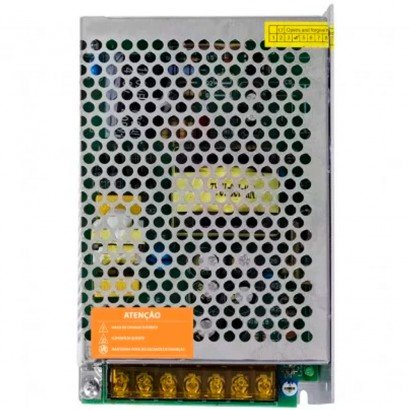
\includegraphics[width=0.4\textwidth]{figuras/fonte_chaveada.jpg}
	\fonte{AMAZON, 2020}
	\label{fig:fontechaveada}
\end{figure} 

\subsection{A motobomba ou bomba d'água}

A bomda d'água selecionada, \autoref{fig:bomba} , trabalha com fontes de alimentação de correntes contínuas (\textit{DC}) o que permite um maior controle do funcionamento através de sistemas \textit{microprocessados}. Essa bomba opera a \textit{12V}, com potência máxima de \textit{80W}. Ela possui a capacidade de exercer uma vazão de \textit{5,5L/min} com ganho de elevação de no máximo 40\textit{m}.

\begin{figure}[H]
	\centering
	\caption{Bomda d'água \textit{DC}}
	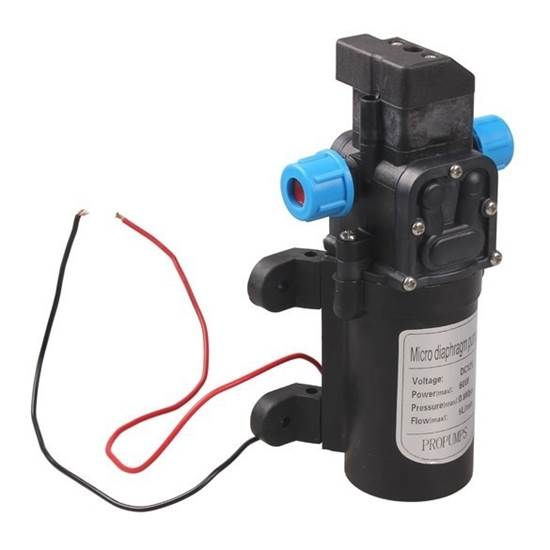
\includegraphics[width=0.3\textwidth]{figuras/bomba.jpeg}
	\fonte{ENERGIA TOTAL, 2020}
	\label{fig:bomba}
\end{figure}

\subsection{O sensor ultrassônico}
\label{ssec:sensor_ultra}

Um sensor ultrassônico é um instrumento que mede a distância até um objeto usando ondas sonoras de frequência acima do alcance da audição humana (ultrassônicas). Ele usa um transdutor para enviar e receber pulsos ultrassônicos os quais são utilizados para medição de distância através de lapsos temporais \autoref{fig:operacao_ultrassonico}.

\begin{figure}[H]
	\centering
	\caption{Representação do funcionamento de um sensor ultrassônico}
	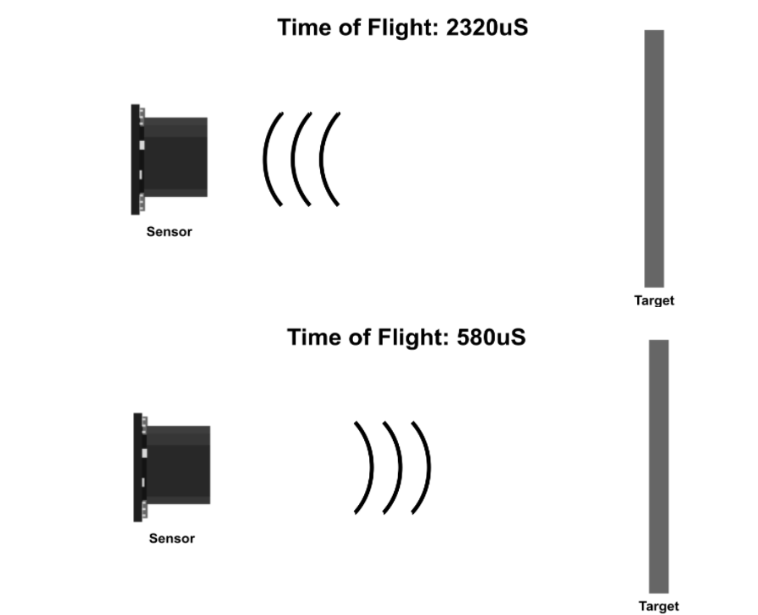
\includegraphics[width=0.6\textwidth]{figuras/ultrassonico_operacao.png}
	\fonte{Maxbotix, 2021}
	\label{fig:operacao_ultrassonico}
\end{figure}

Para medição de nível selecionou-se o módulo ultrassônico \textit{JSN-SR04T}. Esse módulo oferce uma região de medição de distância entre $20 cm$ a $600 cm$, com precisão na faixa de $2 mm$.
Esse módulo inclui um transceptor integrado além do seu circuito de controle.
função de detecção, variando a precisão de até 2 mm; módulo inclui o transceptor de um ultrassônico integrado
sensor e circuito de controle. Modo um de uso e o módulo JSN-SR04T-2.0 da Divisão.
Este produto adota um projeto de sonda ultrassônica integrada de nível industrial, tipo à prova d'água, estável
desempenho, todo o MCU no mercado. 1, o desempenho do módulo é estável, a distância de medição
é preciso. E SRF05, SRF02 estrangeiro e outro módulo telêmetro ultrassônico comparável. Módulo alto
precisão, cego (20cm), gama estável é o produto com sucesso para o mercado uma base forte


O sensor ultrassônico de distância selecionado foi o \textit{JSN-SR04T}, desenvolvido exclusivamente para aperfeiçoar projetos de robótica e microeletrônica, mostrando-se capaz de medir distâncias, em relação a objetos, na faixa entre \textit{25cm} à \textit{150cm}.

\begin{figure}[H]
	\centering
	\caption{Sensor ultrassônico \textit{JSN-SR04T} e módulo de conversão}
	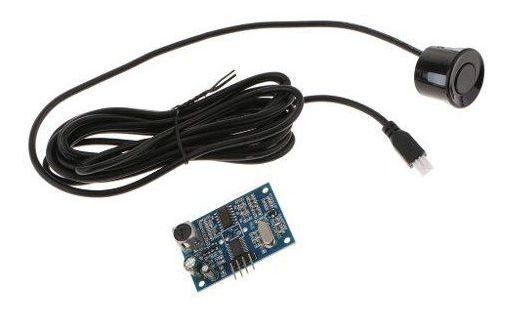
\includegraphics[width=0.5\textwidth]{figuras/sensor_ultra.jpg}
	\fonte{USINAINFO, 2020}
	\label{fig:sensor_ultra}
\end{figure}

O ponto interessante desse sensor é sua ampla e eficiente resistência à umidade, sendo principalmente utilizado em ambientes úmidos, permitindo manter ampla distância do microcontrolador. Ele possui com um fio de \textit{2,5 metros} de comprimento e um módulo especialmente desenvolvido para atuar em conjunto com microcontroladores necessitando de apenas quatro portas de conexão: \textit{5V} (VCC), \textit{Trig (RX)}, \textit{Echo (TX)} e \textit{GND}. Esse sensor apresenta uma eficiência aceitável para a realização da medição de nível


\subsection{A válvula solenoide}

Uma válvula solenoide (\autoref{fig:valvula_solenoide}) é um tipo de válvula que pode ser acionada ou desacionada eletronicamente. Seu componente principal é uma bobina elétrica com um núcleo ferromagnético móvel no centro chamado de êmbolo.

Dependendo a aplicação, uma válvula pode ser classifica em \textbf{Normalmente Aberta - NA} ou\textbf{ Normalmente Fechada - NF}. Para uma \textbf{NF}, em sua posição de repouso, o êmbolo tampa um pequeno orifício por onde é capaz de circular um fluído. Quando uma corrente elétrica circula na bobina, cria um campo magnético o qual exerce força sobre o êmbolo. Ele é deslocado em direção ao centro da bobina, abrindo o orifício e possibilitando a passagem do fluído. A operação para uma válvula \textbf{NA} é justamente o oposto, o êmbolo fica no centro e é deslocado com a formação do campo magnético. Outra classificação é quanto ao número de vias e as formas de controle. Para este trabalho nos atentaremos para válvulas de duas vias com retorno por mola, representadas na figura abaixo.

\begin{figure}[H]
	\centering
	\caption{Representação de válvulas: \textit{(a)} Normalmente Fechada  e \textit{(b)} Normalmente Aberta. Ambas de duas vias.}
	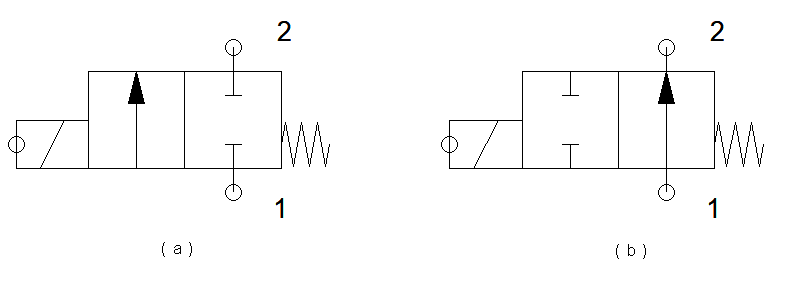
\includegraphics[width=0.7\textwidth]{figuras/valvulas.png}
	\fonte{Própria, 2021}
	\label{fig:valvulas}
\end{figure}

\begin{figure}[H]
	\centering
	\caption{Representação interna de uma válvula solenoide com seus principais componentes}
	\includegraphics[width=0.4\textwidth]{figuras/válvula_solenoide.png}
	\fonte{Citisystems, 2021}
	\label{fig:valvula_solenoide}
\end{figure}

Alguns exemplos do uso de válvula solenoide incluem sistemas de aquecimento, tecnologia de ar comprimido, automação industrial, piscinas, sistemas de aspersão, máquinas de lavar roupa, equipamentos odontológicos, sistemas de lavagem de carros e sistemas de irrigação \cite{Citisystems}.

O modelo de válvula solenoide utilizada foi da marca Nascimetal (\autoref{fig:solenoide}) a qual possui características como:  \textit{1/2"} x \textit{1/2"}, tensão de operação em torno de \textit{12V} \textit{DC}, consumo médio, quando ativada, de \textit{500mA}, pressão de operação à $8,0 kgf/cm^2$ com vazão máxima de $40L/min$ e vida útil de 50 mil operações. Garantiu o controle do fluxo de água de acordo com os dados elétricos enviados pelo microcontrolador.

\begin{figure}[H]
	\centering
	\caption{Válvula solenoide}
	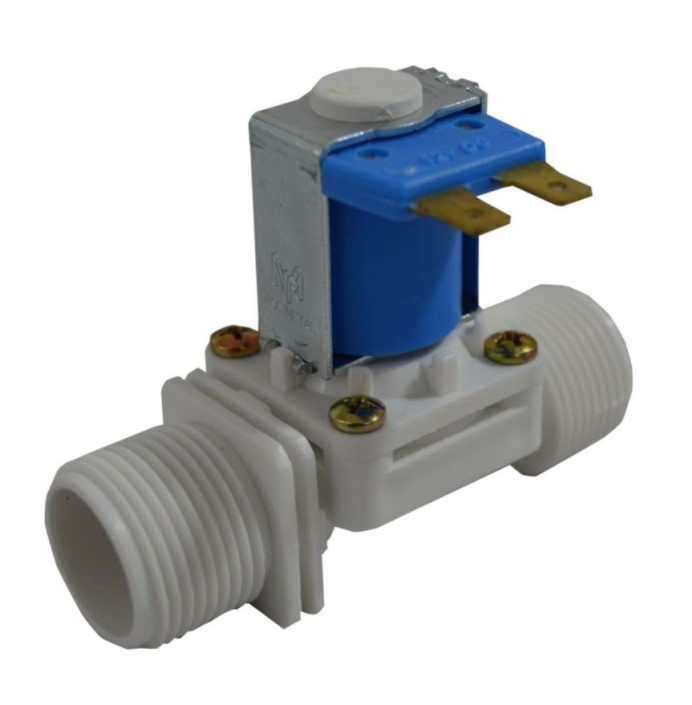
\includegraphics[width=0.3\textwidth]{figuras/solenoide.jpg}
	\fonte{Nascimetal, 2021}
	\label{fig:solenoide}
\end{figure}

\subsection{A chave de nível tipo boia}

Para questões de segurança a chave de nível \textit{RF-0H21D} foi utilizada para fomentar a redundância do sistema, caso aconteçam falhas na medição do sensor citado na seção \ref{ssec:sensor_ultra}. Essa chave indicará para o microcontrolador, por meio de contato elétrico, o momento exato para desativação da bomba d'água, evitando possíveis vazamentos no sistema acolado à caixa d'água (\textbf{TCM}) . 

\begin{figure}[H]
	\centering
	\caption{Chave de nível \textit{RF-0H21D}}
	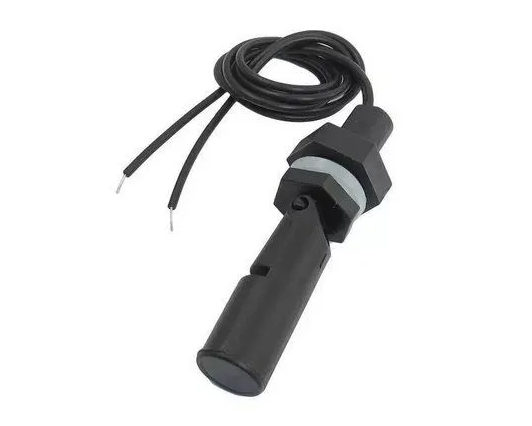
\includegraphics[width=0.5\textwidth]{figuras/chave_boia.png}
	\fonte{SMART KITS, 2020}
	\label{fig:chaveboia}
\end{figure}


\subsection{O sensor de corrente}

O sensor de corrente ACS712 selecionado é barato e oferece precisão em
soluções para detecção de corrente AC ou DC na indústria,
comercial e sistemas de comunicação. O dispositivo permite fácil implementação: aplicações típicas incluem controle de motor, detecção de carga e
gerenciamento, fontes de alimentação comutadas e sobrecorrente
proteção contra falhas.


\begin{figure}[H]
	\centering
	\caption{Representação gráfica do sensor \textit{ACS712}}
	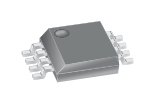
\includegraphics[width=0.3\textwidth]{figuras/ACS712.png}
	\fonte{ALEGRO, 2020}
	\label{fig:acs712}
\end{figure} 


O dispositivo consiste em um operador \textit{Hall} linear preciso, a corrente aplicada flui através do material de cobre gerando um campo magnético que é detectado pelo \textit{Hall} integrado e convertido em um proporcional de tensão. A precisão do dispositivo é otimizada por meio do fechamento proximidade do sinal magnético ao transdutor \textit{Hall}. A resistência interna do material condutor atinge uma média de \textit{1,2m}$\Omega$, proporcionando baixa potência. De acordo \textit{datasheet} do componente, pode-se observar a simples aplicação típica representada na figura abaixo.
 
\begin{figure}[H]
	\centering
	\caption{Aplicação típica do\textit{ACS712}}
	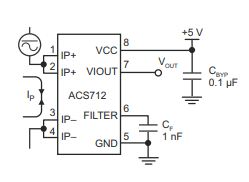
\includegraphics[width=0.4\textwidth]{figuras/ACS712_typical.png}
	\fonte{ALEGRO, 2020}
	\label{fig:acs712_typical}
\end{figure} 


\subsection{KiCad}

O KiCad é o Software de código aberto para projetar circuito eletrônicos. Essa ferramenta EDA - \textit{Electronic Design Automation} lida com captura esquemática e layout de placas de circuito impresso (PCB - \textit{Printed Circuit Board}) gerando arquivos \textit{Gerber} (padrão universal de arquivo composto de uma combinação de comandos gráficos utilizados por equipamentos tipo \textit{fotoploter} para a formação das imagens da placa de circuito impresso).

O Software roda em ambientes Windows, Linux e OS X estando licenciado pela GNU GPL v3. Por meio de sua vasta biblioteca é possível construir esquemáticos de maneira prática. O KiCad também possui recursos de criação e adição de componentes, além de simulação via linguagem SPICE (ainda em beta). 

\begin{figure}[H]
	\centering
	\caption{Exemplo de\textit{PCB Design} utilizando \textit{Kicad}}
	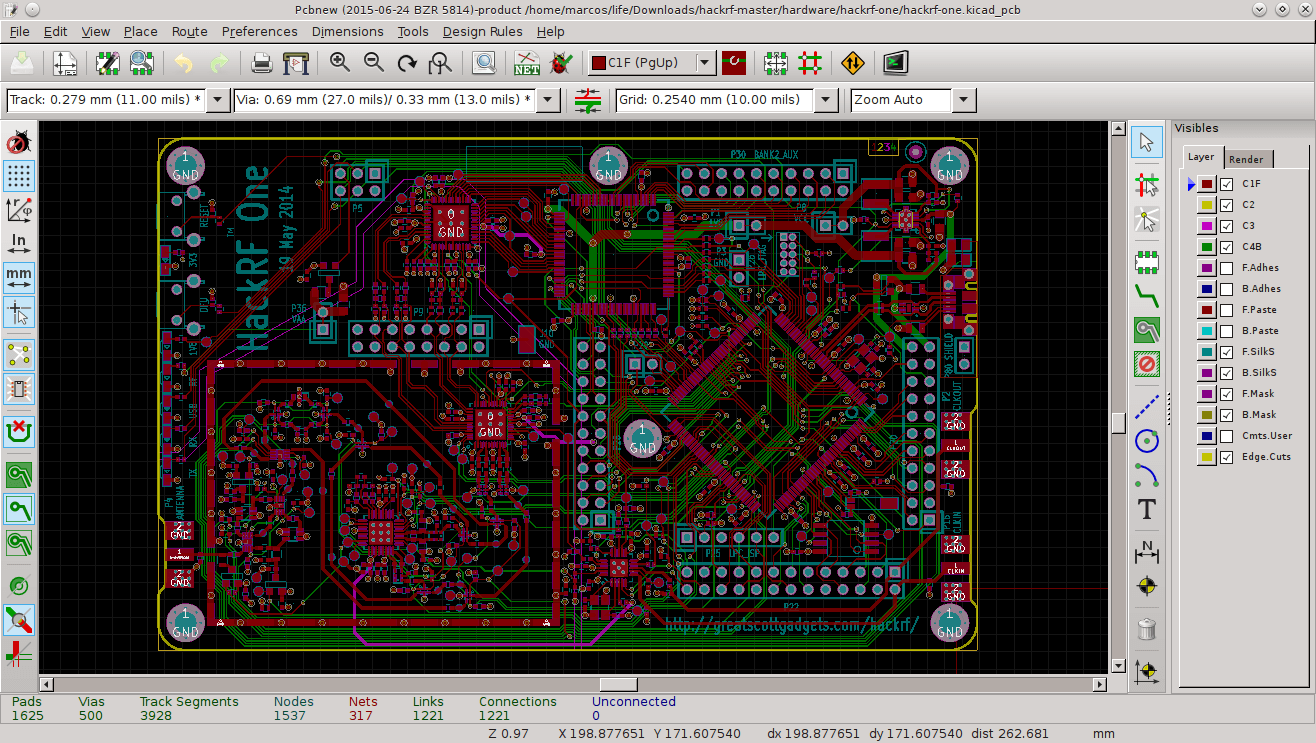
\includegraphics[width=0.6\textwidth]{figuras/kicad_pcbnew.png}
	\fonte{kicad.org, 2021}
	\label{fig:kicad_pcbnew}
\end{figure} 
 

\subsection{Os elementos de ativação e desativação}

Tendo em vista os elementos descritos nos itens anteriores, tornou-se necessário a implementação de um circuito para ativação e desativação da bomba d'água assim como a execução de técnicas de proteção e isolamento.

O diagrama desenvolvido no \textit{software Proteus} (\autoref{fig:diagramaproteus}) mostra a integração de como seria o sistema de ativação e desativação da motobomba.

\begin{figure}[H]
	\centering
	\caption{Diagrama de ativação com partida lenta}
	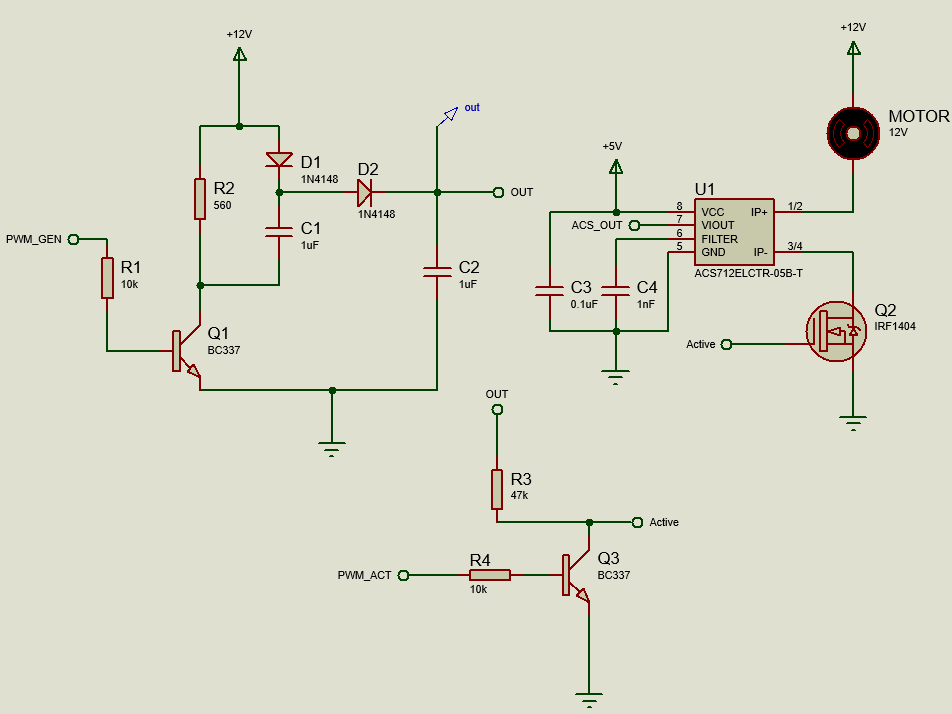
\includegraphics[width=0.9\textwidth]{figuras/diagrama_ativação_bomba.png}
	\fonte{Própria}
	\label{fig:diagramaproteus}
\end{figure} 

A partir deste diagrama utilizou-se técnicas de partida lenta através do chaveamento transistorizado (\textit{BC546}). Por meio do \textit{PWM - Pulse-Width Modulation} oriundo do microcontrolador, o transistor realiza a alteração sobre o valor eficaz de tensão aplicada na bomba d'água.

Para saturação do transistor \textit{IRF1404} (\autoref{fig:IRF1404}) foi desenvolvido o circuito dobrador de tensão também evidenciado na \autoref{fig:diagramaproteus}. A ideia desse circuito é garantir uma queda de tensão entre \textit{GATE} e \textit{SOURCE} duas vezes maior (em torno de \textit{24V}) que a tensão de alimentação do circuito.

\begin{figure}[H]
	\centering
	\caption{Transistor IRF1404}
	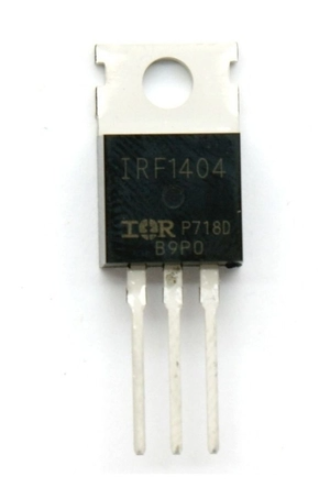
\includegraphics[width=0.2\textwidth]{figuras/IRF1404.png}
	\fonte{ALLDATASHEET, 2020}
	\label{fig:IRF1404}
\end{figure} 



\section{Elementos de \textit{Firmware}}
\subsection{O Ambiente de Desenvolvimento Integrado \textit{Arduino}}

A plataforma Arduino, criada em 2005, não abrange somente as placas microcontroladas mas também agrega-se de uma Interface de Desenvolvimento, ou seja uma IDE, que possui um compilador \textit{C++}. A utilização dessa IDE se tornou tão difundida atualmente que grandes empresas de tecnologia têm buscado tornar ou fabricar microcontroladores completamente compatíveis com a interface.  
Com esta interface, será possível a programação dos microcontroladores \textit{ESP8266} e \textit{ESP32} de maneira facilitada e sem a necessidade do aprendizado de uma nova liguagem. Todas as funcionalidades, como rotinas de conexão \textit{HTTP} e/ou \textit{MQTT} através do \textit{Wi-Fi}, Interrupção, Timers, Modos de Energia são completamente acessíveis. 

\begin{figure}[H]
	\centering
	\caption{Gerenciador de placas com suporte oficial às placas \textit{ESP32} e \textit{ESP8266}}
	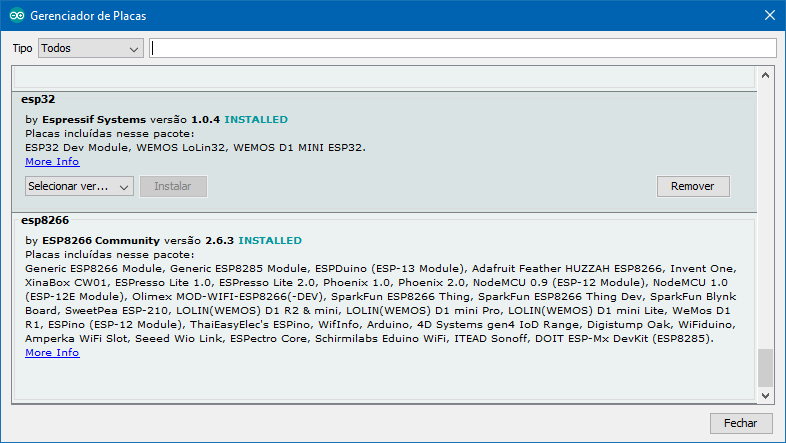
\includegraphics[width=1.0\textwidth]{figuras/gerenciador_placas_arduino.png}
	\fonte{Própria}
	\label{fig:youcto-fluxo}
\end{figure} 

\subsection{Modelagem de um \textit{SO} embarcado com \textit{Yocto Project}}

O \textit{Yocto Project} é um projeto colaborativo de código aberto que fornece modelos, ferramentas e métodos facilitando a criação de sistemas personalizados baseados em Linux para implantações de sistemas embarcados em dispositivos conectados, servidores ou ambientes virtuais, independentemente da arquitetura de hardware.

Por ser um projeto \textit{open source}, opera com uma estrutura de governança hierárquica baseada na meritocracia e gerenciada por seu arquiteto-chefe. Isso permite que o projeto permaneça independente de qualquer um de seus organizadores membros, que participam de várias maneiras e fornecem recursos para o projeto.

O projeto é apoiado e administrado por líderes da indústria de alta tecnologia que se comprometeram financeiramente, com suporte de plataforma e esforços de marketing para tornar o \textit{Yocto Project} um padrão seguro, estável e adaptável da indústria.

\begin{figure}[H]
	\centering
	\caption{Fluxo de trabalho geral \textit{Yocto Project}}
	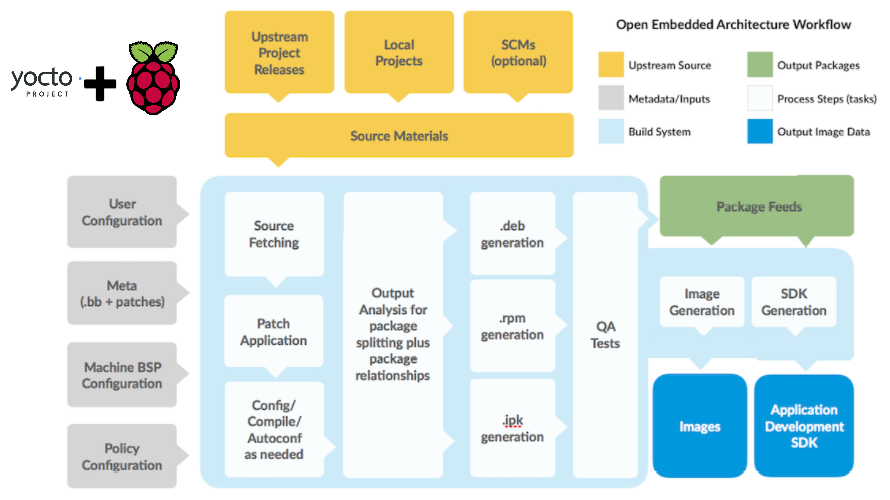
\includegraphics[width=1.0\textwidth]{figuras/yocto-fluxo.png}
	\fonte{Adaptado (yoctoproject.org, 2020)}
	\label{fig:youcto-fluxo}
\end{figure} 

\section{Elementos de \textit{Software}}
\subsection{O \textit{framework React Native}}

Baseado no \textit{React}, para desenvolvimento \textit{WEB}, o \textit{React Native} é um \textit{framework} de codigo aberto desenvolvido pela equipe do \textit{Facebook} que suporta a criação de aplicativos \textit{mobile} multiplataforma (Android e iOS), sem que haja a preocupação de lidar com as linguagens padrões como \textit{Java} ou \textit{Swift}, usando apenas \textit{Javascript}. Como ponto positivo, ao contrário de outros \textit{frameworks} com o mesmo propósito, todo código desenvolvido com \textit{React Native} será convertido para a linguagem nativa do sistema operacional, o que torna o aplicativo mais performático.

\begin{figure}[H]
	\centering
	\caption{Exemplos de \textit{Templates} produzidos com \textit{React Native}}
	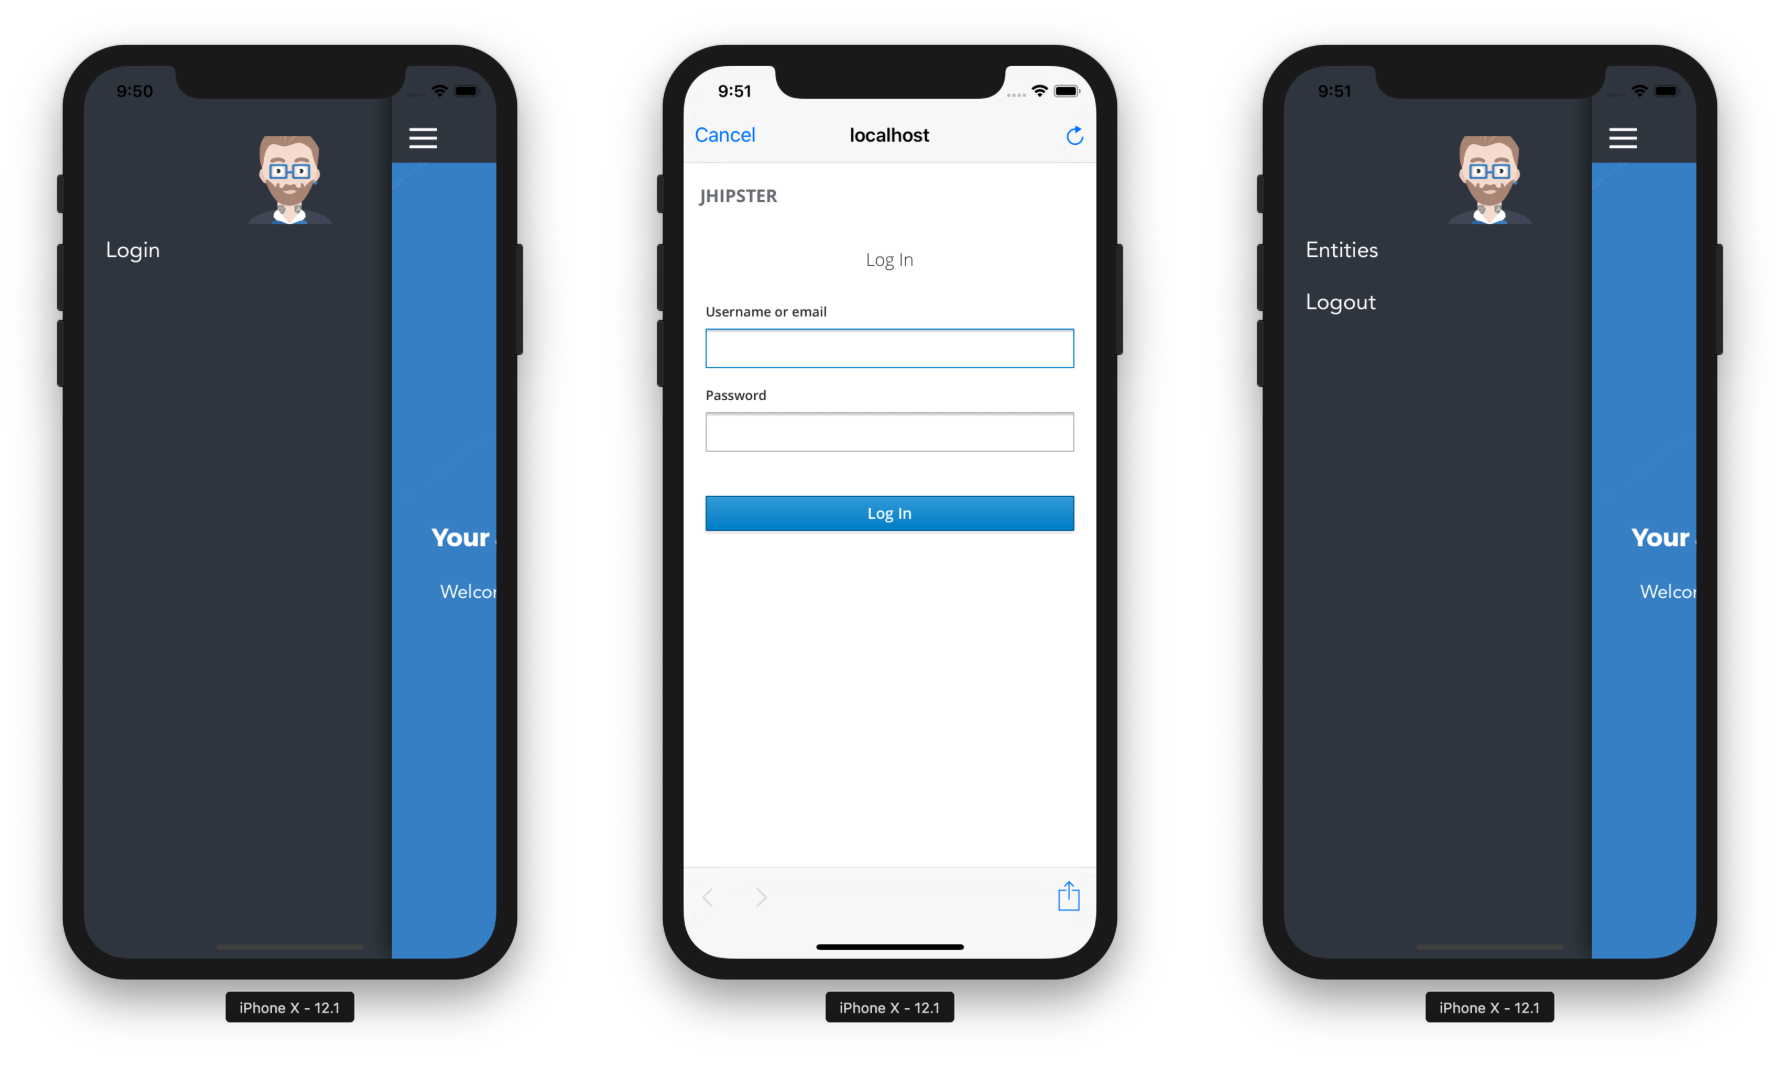
\includegraphics[width=0.7\textwidth]{figuras/react_native_elements.png}
	\fonte{Adaptado (instamobile.io, 2020)}
	\label{fig:youcto-fluxo}
\end{figure} 

\subsection{O \textit{framework Electron}}

O \textit{Electron} é um \textit{framework} multiplataforma (Windows, Linux e MacOS) para criação de interfaces possibilitando o usuário acessar serviços do sistema operacional tanto via linha de comando - \textit{CLI} e interface gráfica - \textit{GUI}.

\begin{figure}[H]
	\centering
	\caption{Aplicações que utilizam \textit{Electron}}
	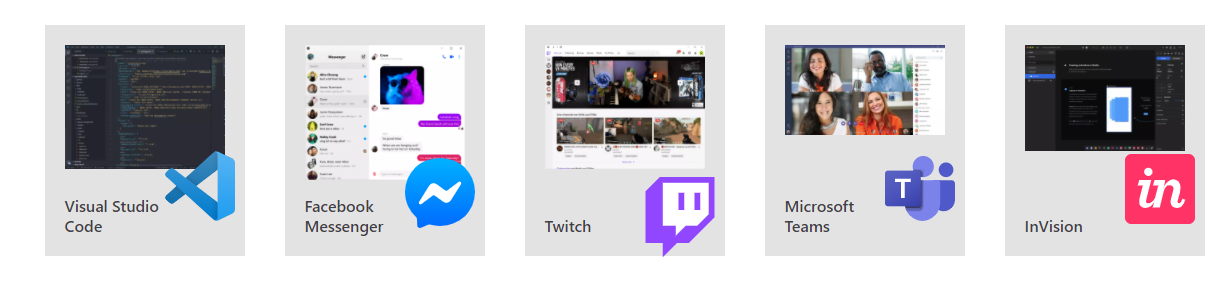
\includegraphics[width=1.0\textwidth]{figuras/electron_apps.png}
	\fonte{Adaptado (electronjs.org, 2020)}
	\label{fig:youcto-fluxo}
\end{figure} 

Por meio dele podemos desenvolver aplicações \textit{desktop} utilizando \textit{HTML}, \textit{CSS} e \textit{Javascript}. O \textit{Electron} vem com navegador \textit{Chromium}, um projeto \textit{open source} de onde surgiu o \textit{Google Chrome}. Toda a parte visual, janelas, etc. são renderizadas nessa camada e o \textit{BackEnd} é executado em \textit{Node.js}. Ambos tem acesso um ao outro via RPC (Remote Procedure Call).



